%% 
%% Copyright 2007-2020 Elsevier Ltd
%% 
%% This file is part of the 'Elsarticle Bundle'.
%% ---------------------------------------------
%% 
%% It may be distributed under the conditions of the LaTeX Project Public
%% License, either version 1.2 of this license or (at your option) any
%% later version.  The latest version of this license is in
%%    http://www.latex-project.org/lppl.txt
%% and version 1.2 or later is part of all distributions of LaTeX
%% version 1999/12/01 or later.
%% 
%% The list of all files belonging to the 'Elsarticle Bundle' is
%% given in the file `manifest.txt'.
%% 
%% Template article for Elsevier's document class `elsarticle'


\documentclass[preprint,12pt,authoryear]{elsarticle}

%% Use the option review to obtain double line spacing
%% \documentclass[authoryear,preprint,review,12pt]{elsarticle}

%% For including figures, graphicx.sty has been loaded in
%% elsarticle.cls. If you prefer to use the old commands
%% please give \usepackage{epsfig}

%% The amssymb package provides various useful mathematical symbols
\usepackage{amssymb}
\linespread{1.2}

%% The amsthm package provides extended theorem environments
%% \usepackage{amsthm}

%% The lineno packages adds line numbers. Start line numbering with
%% \begin{linenumbers}, end it with \end{linenumbers}. Or switch it on
%% for the whole article with \linenumbers.

\usepackage{lineno}
\usepackage{graphicx}
\usepackage[colorlinks=true, allcolors=blue]{hyperref}

% SI numbering
\renewcommand\thefigure{S\arabic{figure}}
\renewcommand\thetable{S\arabic{table}}
\setcounter{figure}{0}
\setcounter{table}{0}

\journal{Estuaries and Coasts}

\begin{document}

\begin{frontmatter}

%% Title, authors and addresses

%% use the tnoteref command within \title for footnotes;
%% use the tnotetext command for theassociated footnote;
%% use the fnref command within \author or \affiliation for footnotes;
%% use the fntext command for theassociated footnote;
%% use the corref command within \author for corresponding author footnotes;
%% use the cortext command for theassociated footnote;
%% use the ead command for the email address,
%% and the form \ead[url] for the home page:
%% \title{Title\tnoteref{label1}}
%% \tnotetext[label1]{}
%% \author{Name\corref{cor1}\fnref{label2}}
%% \ead{email address}
%% \ead[url]{home page}
%% \fntext[label2]{}
%% \cortext[cor1]{}
%% \affiliation{organization={},
%%            addressline={}, 
%%            city={},
%%            postcode={}, 
%%            state={},
%%            country={}}
%% \fntext[label3]{}

\title{Supporting Information for ``Seepage across the berm of an intermittently closed estuary'' }

%% use optional labels to link authors explicitly to addresses:
\author[ars]{Octavia Crompton}
\affiliation[ars]{
            organization={USDA-ARS Hydrology and Remote Sensing Laboratory},
            % addressline={},
            % city={},
            % postcode={},
            % state={},
            % country={}
            }

\author[bml]{John Largier}
\affiliation[bml]{
            organization={UC Davis Bodega Bay Marine Lab},
            % addressline={},
            % city={},
            % postcode={},
            % state={},
            % country={}
            }
            
%%
%% \affiliation[label2]{organization={},
%%             addressline={},
%%             city={},
%%             postcode={},
%%             state={},
%%             country={}}

\author[esa]{Dane Behrens}

\affiliation[esa]{organization=
            {Environmental Science Associates},
            % addressline={}, 
            % city={},
            % postcode={}, 
            % state={},
            % country={}
            }


\end{frontmatter}

%% \linenumbers

\newpage

  \begin{figure}
    \centering
    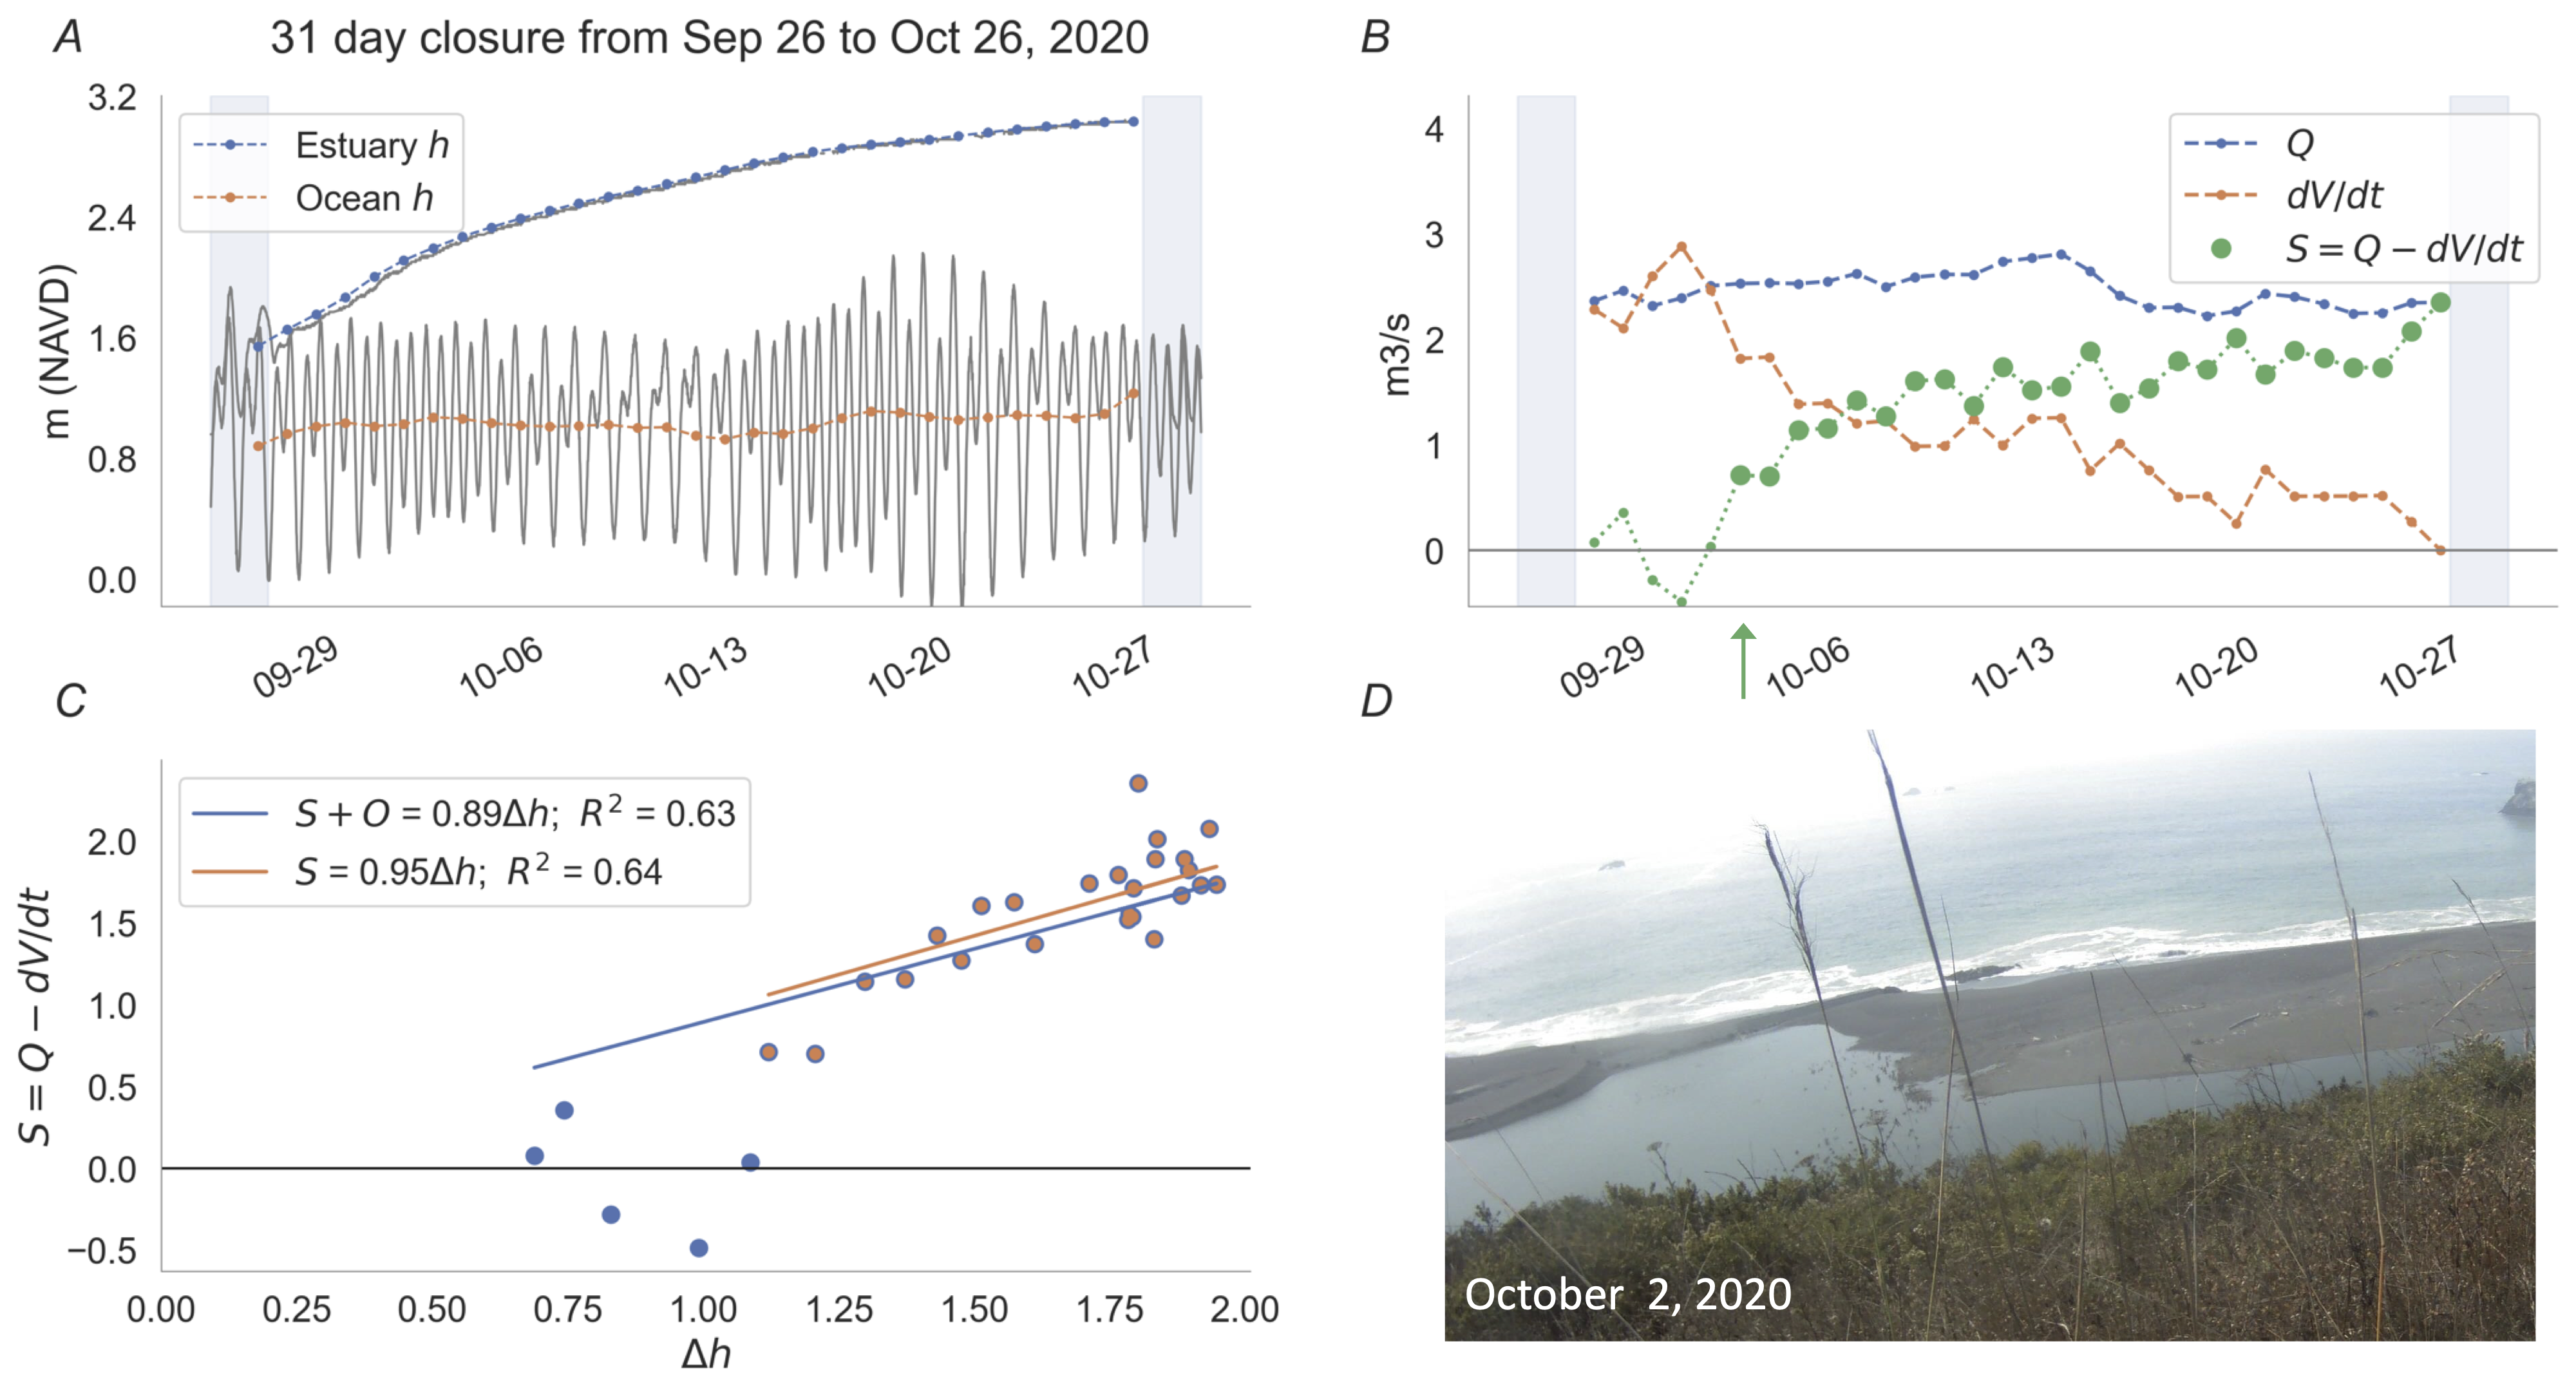
\includegraphics[width = \textwidth]{figures/closure2.png}
    \caption{(A) Timeseries of estuary depth and ocean level at Pt. Reyes during a closure from September 26, 2020  - October 26, 2020.
    Solid lines show 15 minute data, and dotted lines show the daily averaged.
    Grey shading indicates periods when the estuary was open.
    (B)  The mass balance components of mass balance at daily intervals: the estuary volume change per day, $dV/dt$  (orange),  river discharge, $Q_r$  (blue) and seepage, $S = Q - dV/dt$ (green). No markers where data filtered to avoid overwash. 
     (C) The berm integrated hydraulic conductivity $\tilde K$ was computed by fitting a regression of $S$ on $\Delta h$.
    (D) Visual inspection of an estuary photo taken September 15, 2014, illustrating overwash. 
    }
    \label{fig:timeseries}
\end{figure}


  \begin{figure}
    \centering
    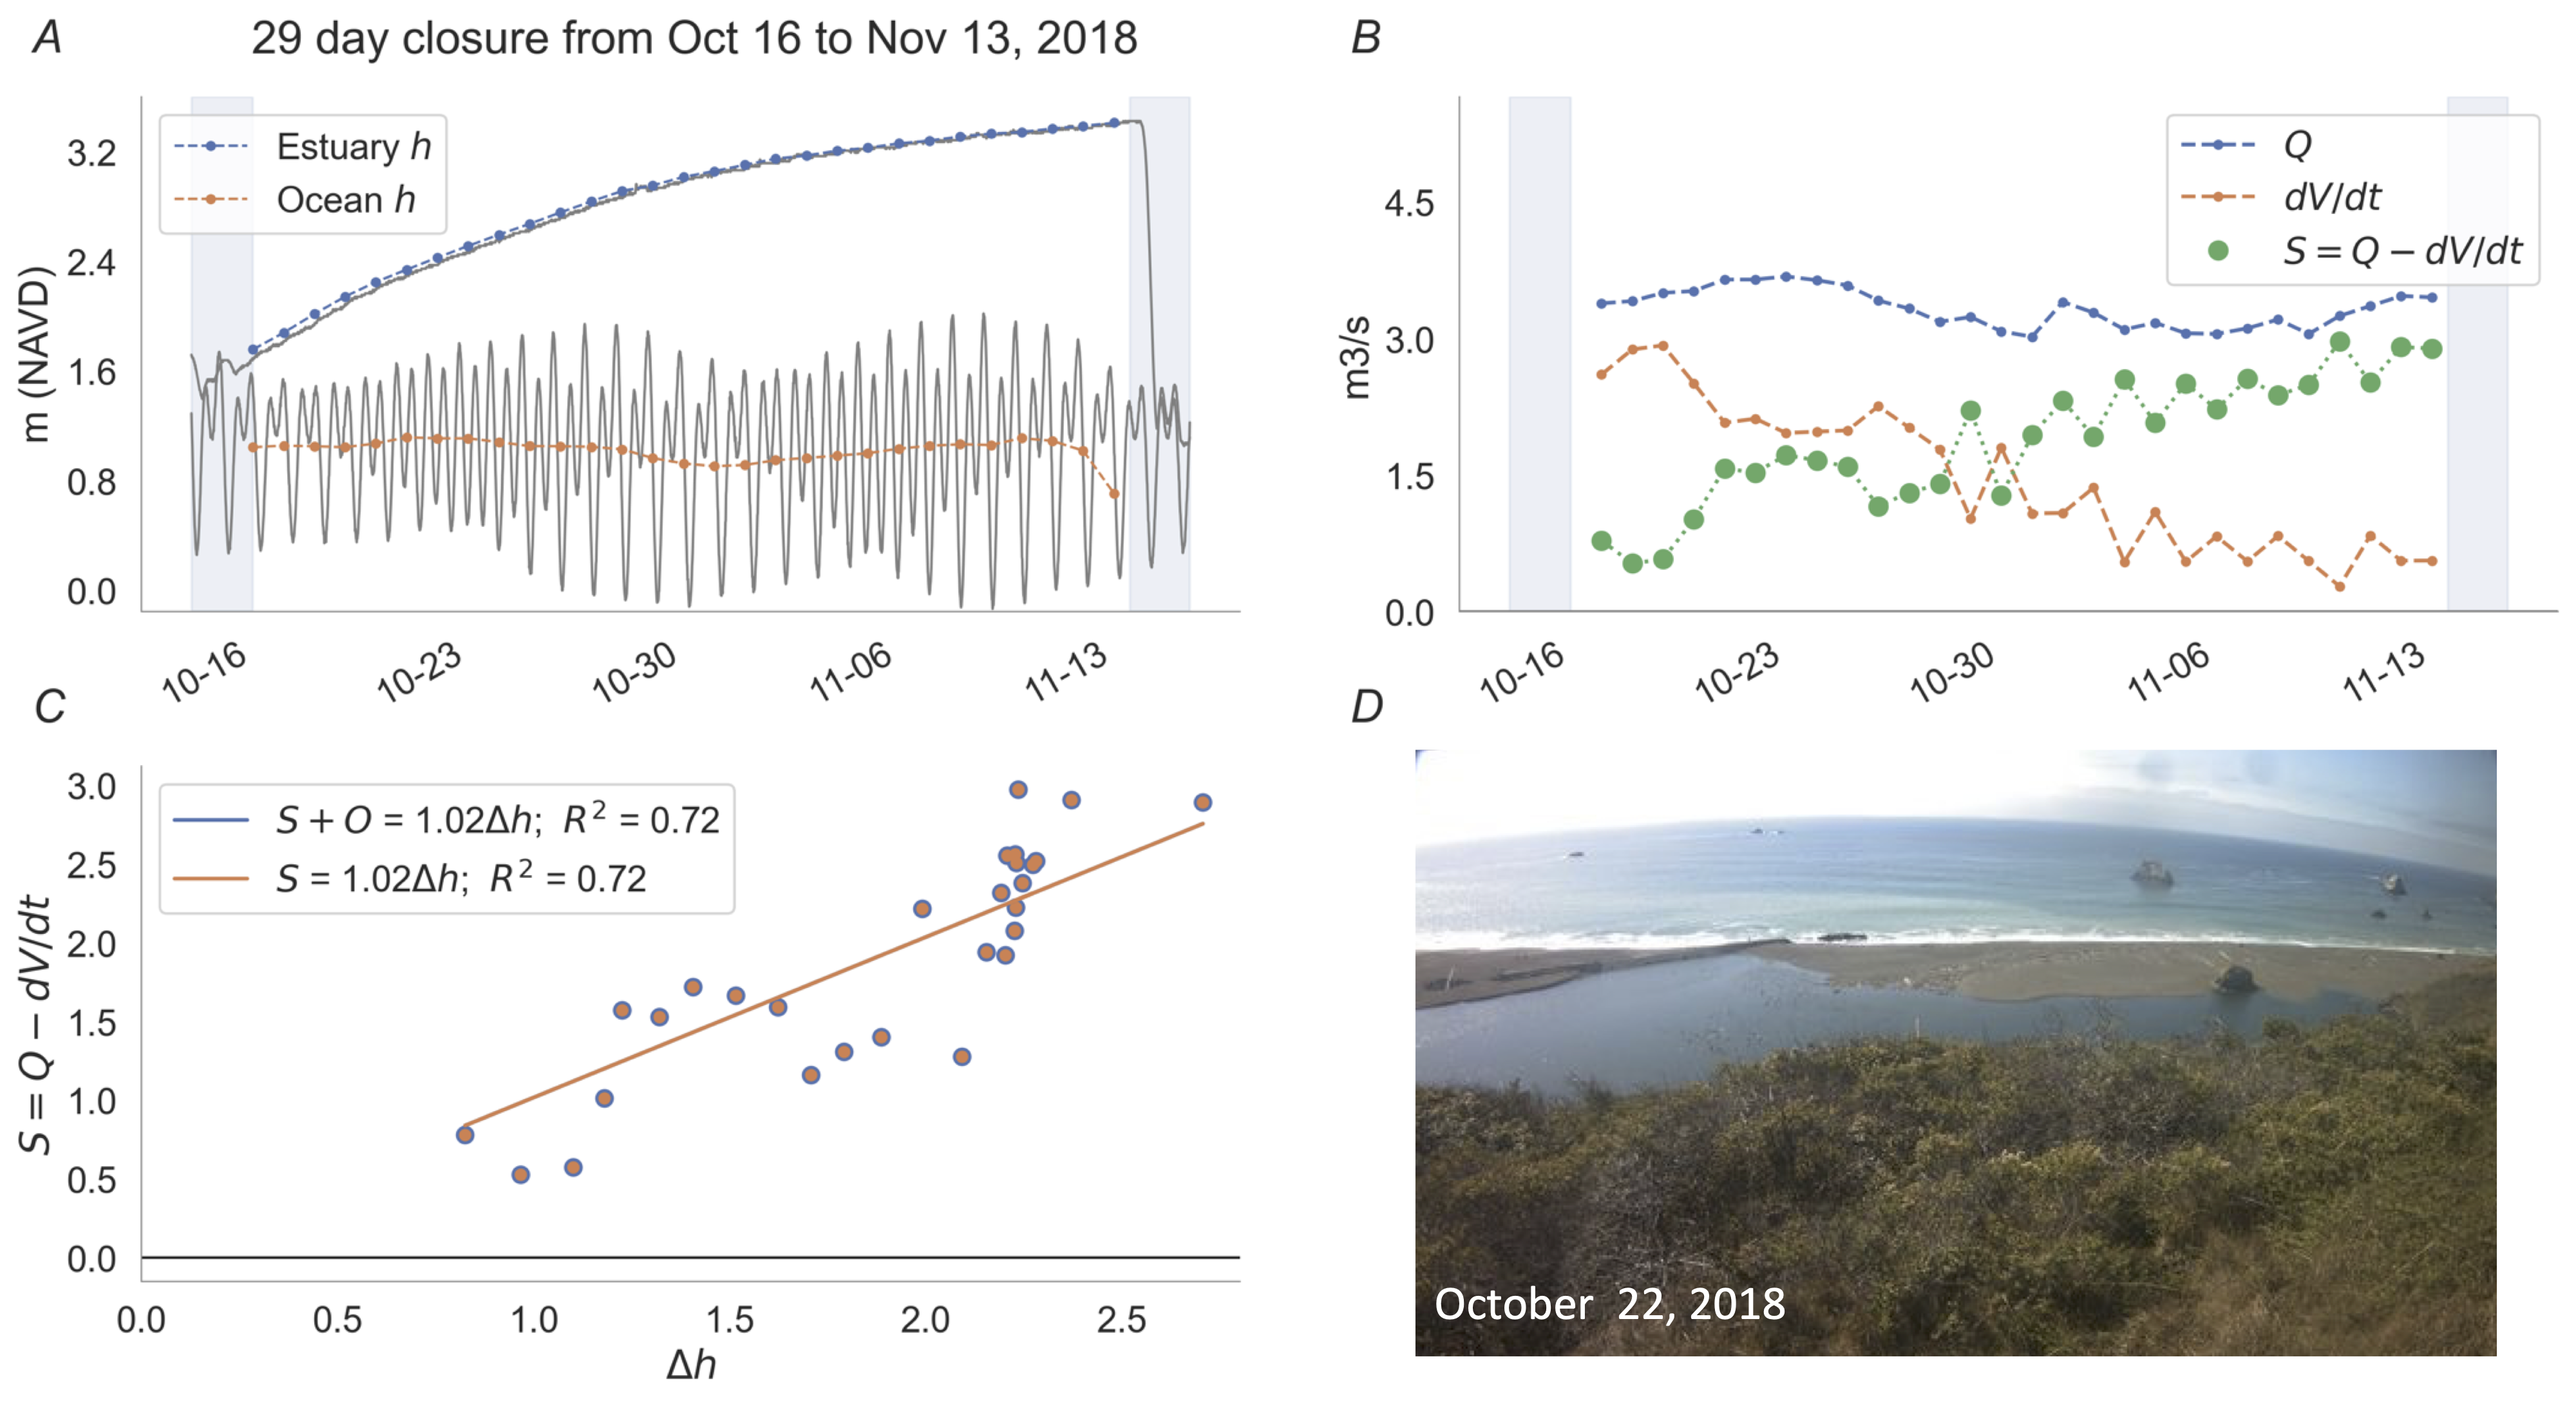
\includegraphics[width = \textwidth]{figures/closure3.png}
    \caption{(A) Timeseries of estuary depth and ocean level at Pt. Reyes during a closure from October 16, 2018, - November 13, 2018.
    Solid lines show 15 minute data, and dotted lines show the daily averaged.
    Grey shading indicates periods when the estuary was open.
    (B)  The mass balance components of mass balance at daily intervals: the estuary volume change per day, $dV/dt$  (orange),  river discharge, $Q_r$  (blue) and seepage, $S = Q - dV/dt$ (green). No markers where data filtered to avoid overwash. 
     (C) The berm integrated hydraulic conductivity $\tilde K$ was computed by fitting a regression of $S$ on $\Delta h$.
    (D) Visual inspection of an estuary photo taken September 15, 2014, illustrating overwash. 
    }
    \label{fig:timeseries}
\end{figure}

\begin{figure}[h]
    \centering
    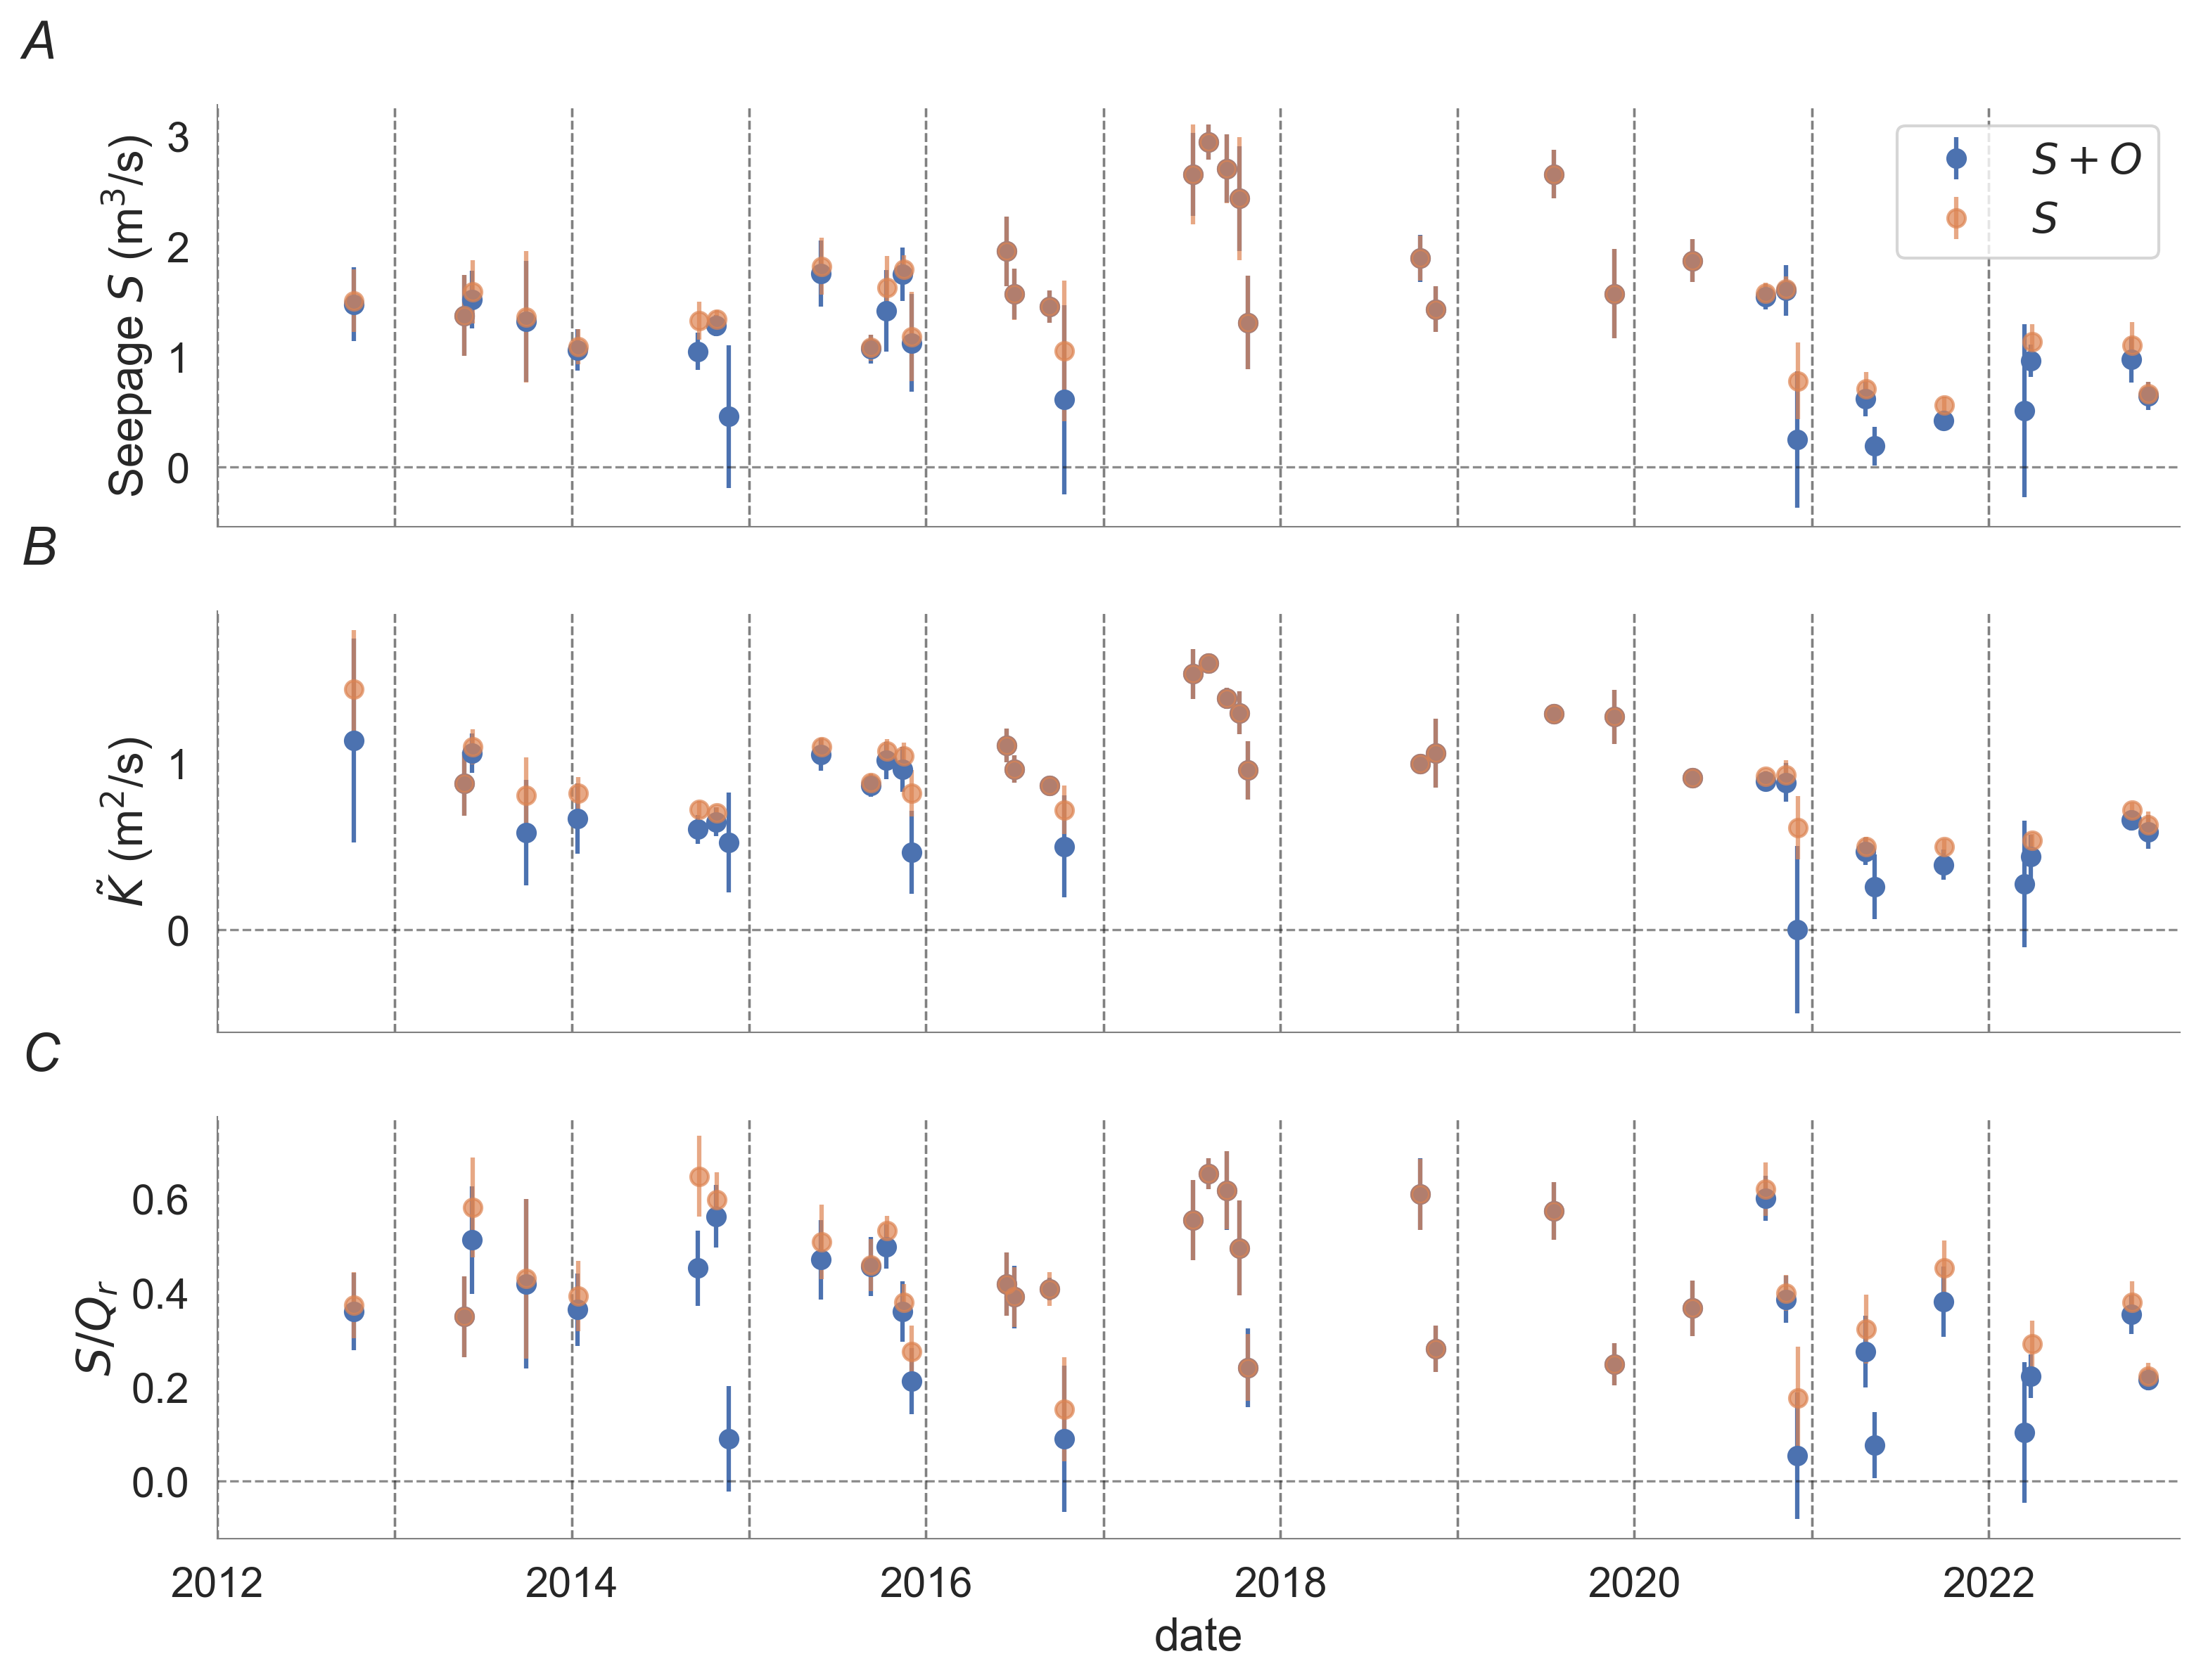
\includegraphics[width = 30pc]{figures/summary_w_overwash.png}
    \caption{(A) Median seepage rates computed for each closure, with error bars showing bootstrapped confidence intervals.
    (B) Integrated hydraulic conductivity determined through regression of $S$ on $\Delta h$ for each closure event.  
    (C) Ratio of seepage to discharge, $S/Q_r$. 
    Only events with at least 5 days of data are included.  
    }
    \label{fig:summary}
\end{figure}



\end{document}

\endinput
%%

